% Provenance (never printed): the demand-and-supply strand of ../economics_series.md (grade 7: tables, curves,
% the meeting point; the model box is in g9-01). Brief: sources/book1/BRIEFS.md, g7-06. Chart data:
% figdata/grade-7/06-demand-and-supply-first-look (BLS average prices, strawberries; invented Brenmoor tables).
\chapter{Demand and Supply: A First Look}\label{ch:g7:demand-and-supply-first-look}

\begin{openingchart}{Average price of a 12-ounce pint of strawberries in shops in the
United States, each month of 2022, 2023 and 2024, in dollars.}{U.S. Bureau of Labor
Statistics, average \omterm{def:g7:money:price}{price} data, strawberries, dry pint, per 12 oz., U.S. city average}
\begin{tikzpicture}
\begin{axis}[omrecord, xmin=1, xmax=12, ymin=0, ymax=4.5, xtick={1,...,12},
  xticklabels={Jan, Feb, Mar, Apr, May, Jun, Jul, Aug, Sep, Oct, Nov, Dec},
  ylabel={Dollars per pint},
  legend style={at={(0.5,-0.15)}, anchor=north, legend columns=3}]
\pgfplotsforeachungrouped \col in {y2022, y2023, y2024} {
  \addplot table[x=month, y=\col] {figdata/grade-7/06-demand-and-supply-first-look/out/strawberry_months.csv};
}
\legend{2022, 2023, 2024}
\end{axis}
\end{tikzpicture}
\end{openingchart}

% figdata: facts (y2022 min 2.21 in July, max 3.86 in December; y2023 min 2.42 in July, max 3.57 in December;
% y2024 min 2.06 in June, max 3.66 in January)
Every year, strawberries are cheapest in early summer and dearest in winter. In 2024, a
pint cost $3.66$ dollars in January and $2.06$ dollars in June; in 2023, $2.42$ dollars in
July and $3.57$ dollars in December. The three years draw almost the same curve. Early
summer is when the fields of many regions are being picked at once; in winter, strawberries
come from a few warm regions or from greenhouses, at a higher cost.

The chart shows only \omterm{def:g7:money:price}{prices}. To understand them, one must look at both sides of the
\omterm{def:g7:markets-and-prices:market}{market}: how much buyers want at each \omterm{def:g7:money:price}{price}, and how much sellers bring. This chapter
draws these two plans as tables and as curves, and finds the \omterm{def:g7:money:price}{price} at which they meet.

\begin{recall}
The \omterm{def:g7:markets-and-prices:market-price}{market price} is the \omterm{def:g7:money:price}{price} at which buyers and sellers actually exchange; at a \omterm{def:g7:money:price}{price}
where buyers want more than sellers offer, there is a \omterm{def:g7:markets-and-prices:shortage}{shortage}; in the opposite case, a
\omterm{def:g7:markets-and-prices:market-surplus}{market surplus} (\cref{ch:g7:markets-and-prices}).
\end{recall}

\begin{omfigure}
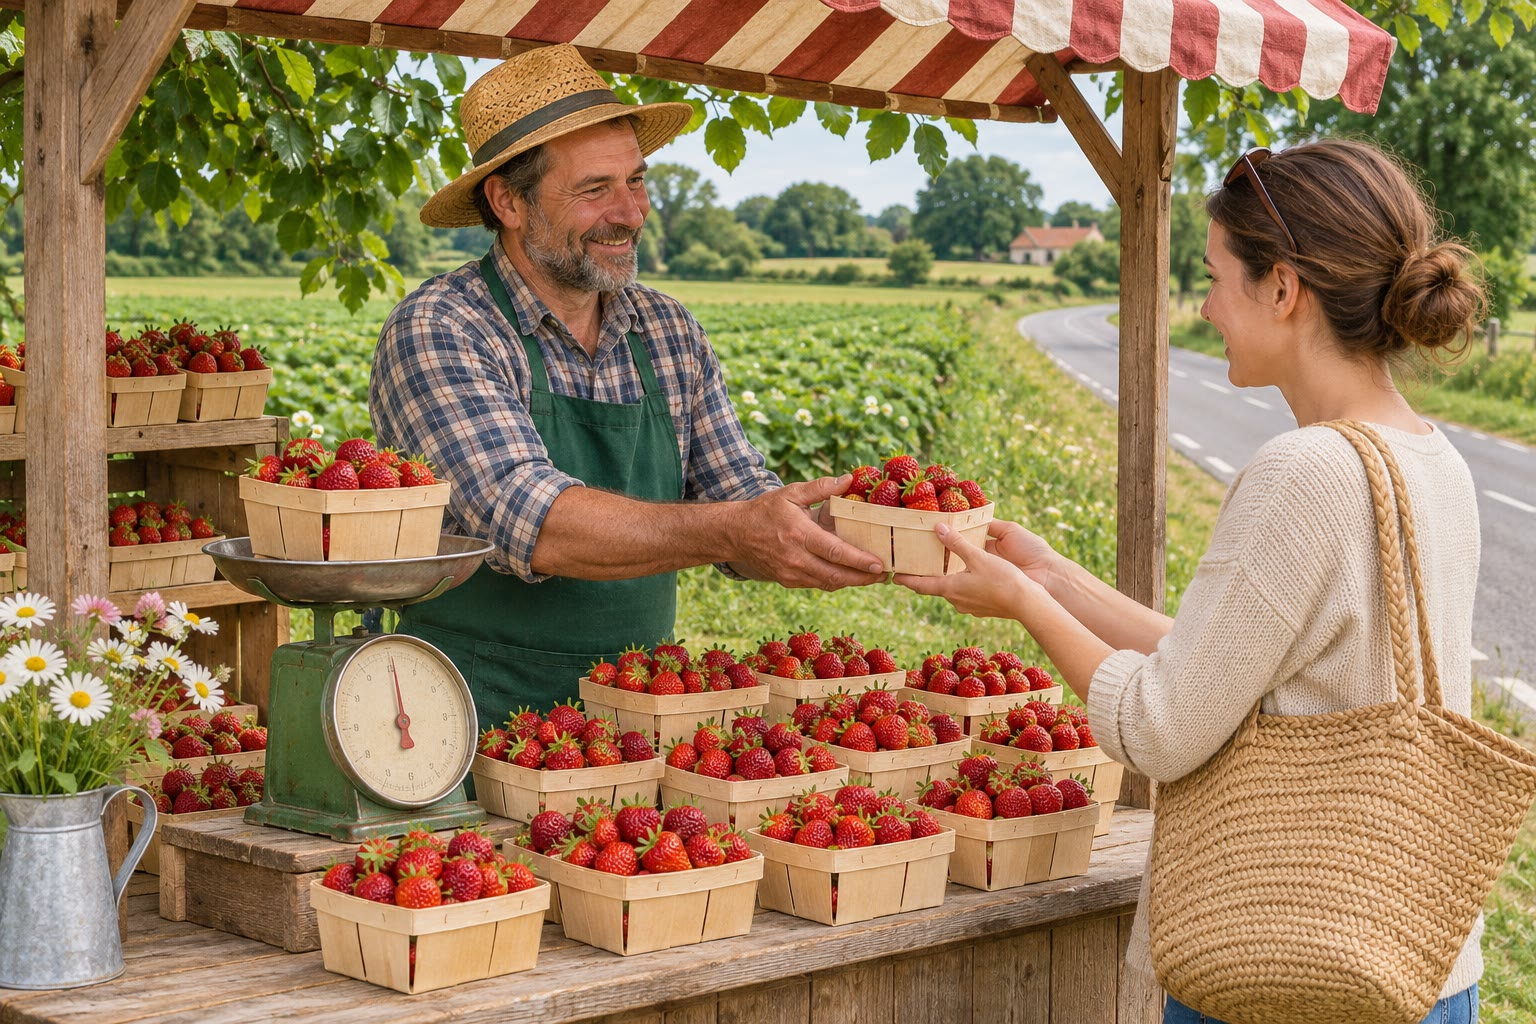
\includegraphics[width=0.52\linewidth]{images/book1/ai/g7-demand-and-supply-first-look-strawberries.jpg}

{\small A strawberry stall in early summer. At this time of the year, the fields are full
and the baskets cheap.}
\end{omfigure}

\section{A demand table and its curve}

\begin{definition}[Quantity demanded]\label{def:g7:demand-and-supply-first-look:quantity-demanded}
The \emph{quantity demanded}\index{quantity demanded} of a good, at a given \omterm{def:g7:money:price}{price}, is the
quantity that buyers want to buy and can pay for at that \omterm{def:g7:money:price}{price}, in a given time.
\end{definition}

\begin{definition}[Demand table]\label{def:g7:demand-and-supply-first-look:demand-table}
A \emph{demand table}\index{demand table} lists, for several \omterm{def:g7:money:price}{prices}, the \omterm{def:g7:demand-and-supply-first-look:quantity-demanded}{quantity demanded}
at each, all other things staying the same.
\end{definition}

\begin{measure}[Quantity demanded is a plan]
A \omterm{def:g7:demand-and-supply-first-look:quantity-demanded}{quantity demanded} is not what was bought: it is what buyers \emph{would} buy at a \omterm{def:g7:money:price}{price}.
Only one \omterm{def:g7:money:price}{price} happens at a time, so only one point of a \omterm{def:g7:demand-and-supply-first-look:demand-table}{demand table} is ever seen in the
shops. Economists estimate the others by watching how quantities bought change when \omterm{def:g7:money:price}{prices}
change for reasons that have nothing to do with buyers, or by surveys and experiments.
\end{measure}

The households of Brenmoor buy strawberries at the town \omterm{def:g7:markets-and-prices:market}{market}. The table, invented for
this chapter, gives their weekly plans in May and those of the growers.

% figdata: berry_tables (price 1..5; demanded 1000 800 600 400 200; supplied 200 400 600 800 1000)
\begin{center}
\begin{tabular}{lccccc}
\toprule
\omterm{def:g7:money:price}{Price} (dalens per basket) & 1 & 2 & 3 & 4 & 5 \\
\midrule
\omterm{def:g7:demand-and-supply-first-look:quantity-demanded}{Quantity demanded} (baskets a week) & 1\,000 & 800 & 600 & 400 & 200 \\
\omterm{def:g7:demand-and-supply-first-look:quantity-supplied}{Quantity supplied} (baskets a week) & 200 & 400 & 600 & 800 & 1\,000 \\
\bottomrule
\end{tabular}
\end{center}

\begin{definition}[Demand curve]\label{def:g7:demand-and-supply-first-look:demand-curve}
A \emph{demand curve}\index{demand curve} is the graph of a \omterm{def:g7:demand-and-supply-first-look:demand-table}{demand table}: the \omterm{def:g7:money:price}{price} on the
vertical axis, the \omterm{def:g7:demand-and-supply-first-look:quantity-demanded}{quantity demanded} on the horizontal axis, one point for each line of the
table, joined.
\end{definition}

The higher the \omterm{def:g7:money:price}{price}, the fewer baskets the households want: the \omterm{def:g7:demand-and-supply-first-look:demand-curve}{demand curve} goes down
from left to right. At a high \omterm{def:g7:money:price}{price} some households buy fewer baskets, others none, and
others turn to cherries or apples.

\section{A supply table and its curve}

\begin{definition}[Quantity supplied]\label{def:g7:demand-and-supply-first-look:quantity-supplied}
The \emph{quantity supplied}\index{quantity supplied} of a good, at a given \omterm{def:g7:money:price}{price}, is the
quantity that sellers want to sell at that \omterm{def:g7:money:price}{price}, in a given time.
\end{definition}

\begin{definition}[Supply table]\label{def:g7:demand-and-supply-first-look:supply-table}
A \emph{supply table}\index{supply table} lists, for several \omterm{def:g7:money:price}{prices}, the \omterm{def:g7:demand-and-supply-first-look:quantity-supplied}{quantity supplied}
at each, all other things staying the same.
\end{definition}

\begin{definition}[Supply curve]\label{def:g7:demand-and-supply-first-look:supply-curve}
A \emph{supply curve}\index{supply curve} is the graph of a \omterm{def:g7:demand-and-supply-first-look:supply-table}{supply table}, with the \omterm{def:g7:money:price}{price} on
the vertical axis and the \omterm{def:g7:demand-and-supply-first-look:quantity-supplied}{quantity supplied} on the horizontal axis.
\end{definition}

The higher the \omterm{def:g7:money:price}{price}, the more baskets the growers bring: they pick the less ripe corners of
their fields, hire more pickers, and some growers who sell elsewhere come to Brenmoor. The
\omterm{def:g7:demand-and-supply-first-look:supply-curve}{supply curve} goes up from left to right.

\begin{omchart}{The demand and supply tables of the Brenmoor strawberry market in May,
drawn as curves (invented data).}{The chapter's invented example}
\begin{tikzpicture}
\begin{axis}[omrecord, xmin=0, xmax=1200, ymin=0, ymax=6, xtick={0,200,...,1200},
  ytick={0,...,6}, xlabel={Baskets a week}, ylabel={Dalens per basket},
  height=0.55\linewidth, width=0.7\linewidth, legend pos=north east]
\addplot[demand, mark=*, mark size=1.6pt] table[x=demanded, y=price]
  {figdata/grade-7/06-demand-and-supply-first-look/out/berry_tables.csv};
\addplot[supply, mark=square*, mark size=1.5pt] table[x=supplied, y=price]
  {figdata/grade-7/06-demand-and-supply-first-look/out/berry_tables.csv};
\legend{Demand, Supply}
\end{axis}
\end{tikzpicture}
\end{omchart}

\section{Where they meet}

\begin{definition}[Equilibrium price]\label{def:g7:demand-and-supply-first-look:equilibrium-price}
The \emph{equilibrium price}\index{equilibrium price} is the \omterm{def:g7:money:price}{price} at which the \omterm{def:g7:demand-and-supply-first-look:quantity-demanded}{quantity
demanded} equals the \omterm{def:g7:demand-and-supply-first-look:quantity-supplied}{quantity supplied}.
\end{definition}

\begin{definition}[Equilibrium quantity]\label{def:g7:demand-and-supply-first-look:equilibrium-quantity}
The \emph{equilibrium quantity}\index{equilibrium quantity} is the quantity bought and sold
at the \omterm{def:g7:demand-and-supply-first-look:equilibrium-price}{equilibrium price}.
\end{definition}

In the table, the two quantities match at 3 dalens: 600 baskets are wanted and 600 offered.
On the graph, the equilibrium is the point where the two curves cross, at a \omterm{def:g7:money:price}{price} of 3
dalens and a quantity of 600 baskets.

\section{Above and below the meeting price}

At 4 dalens, growers bring 800 baskets and households want 400: a \omterm{def:g7:markets-and-prices:market-surplus}{market surplus} of 400
baskets. Growers left with baskets lower their \omterm{def:g7:money:price}{price}. At 2 dalens, households want 800
baskets and growers bring 400: a \omterm{def:g7:markets-and-prices:shortage}{shortage} of 400. Households who find no strawberries offer
more, and growers raise the \omterm{def:g7:money:price}{price}. Only at 3 dalens does nobody have a reason to change the
\omterm{def:g7:money:price}{price}. This is why the \omterm{def:g7:markets-and-prices:market-price}{market price} is usually close to the \omterm{def:g7:demand-and-supply-first-look:equilibrium-price}{equilibrium price}.

\section{When a curve moves}

A \omterm{def:g7:demand-and-supply-first-look:demand-table}{demand table} is drawn ``all other things staying the same''. When one of those other
things changes, the whole table changes, and the curve moves.

\begin{definition}[Shift of a curve]\label{def:g7:demand-and-supply-first-look:shift}
A \emph{shift}\index{shift of a curve} of a demand or \omterm{def:g7:demand-and-supply-first-look:supply-curve}{supply curve} is a change of the
\omterm{def:g7:demand-and-supply-first-look:quantity-demanded}{quantity demanded} or supplied \emph{at every \omterm{def:g7:money:price}{price}}, caused by something other than the
good's own \omterm{def:g7:money:price}{price}.
\end{definition}

The \omterm{def:g7:demand-and-supply-first-look:demand-curve}{demand curve} \omterm{def:g7:demand-and-supply-first-look:shift}{shifts} when buyers' tastes, incomes, the number of buyers or the \omterm{def:g7:money:price}{prices} of
other goods change. The \omterm{def:g7:demand-and-supply-first-look:supply-curve}{supply curve} \omterm{def:g7:demand-and-supply-first-look:shift}{shifts} when the costs of growing, the weather, the
number of growers or the tools change. A change in the good's own \omterm{def:g7:money:price}{price} does not \omterm{def:g7:demand-and-supply-first-look:shift}{shift} a
curve: it moves along it.

\begin{example}
In the last week of May, a heat wave makes the households of Brenmoor want 400 more baskets
at every \omterm{def:g7:money:price}{price}: 1\,400 at 1 dalen, 1\,200 at 2, 1\,000 at 3, 800 at 4, 600 at 5. At the old
\omterm{def:g7:money:price}{price} of 3 dalens, 1\,000 baskets are now wanted and 600 offered: a \omterm{def:g7:markets-and-prices:shortage}{shortage} of 400. The
\omterm{def:g7:money:price}{price} rises. At 4 dalens, 800 baskets are wanted and 800 offered: the new equilibrium is 4
dalens and 800 baskets.
\end{example}

\begin{omfigure}
\begin{tikzpicture}[econ, x=0.8cm, y=0.8cm]
  % 1 unit = 200 baskets on x, 1 dalen on y: demand y = 6 - x, supply y = x, shifted demand y = 8 - x
  \draw[econ axes] (0,6.6) node[above, font=\scriptsize] {dalens per basket} |- (8.6,0)
    node[right, font=\scriptsize] {baskets};
  \foreach \x/\l in {1/200, 2/400, 3/600, 4/800, 5/1000, 6/1200, 7/1400}
    \draw (\x,0) -- (\x,-0.1) node[below, font=\scriptsize] {\l};
  \foreach \y in {1,...,6} \draw (0,\y) -- (-0.1,\y) node[left, font=\scriptsize] {\y};
  \draw[supply] (0,0) -- (6.3,6.3) node[above right, font=\scriptsize] {supply};
  \draw[demand] (0,6) -- (6,0);
  \node[omDef, font=\scriptsize, align=left, anchor=west] at (5.55,0.6) {demand\\in May};
  \draw[demand, shifted] (2,6) -- (8,0);
  \node[omDef, font=\scriptsize, align=left, anchor=west] at (7.0,1.35) {demand after\\the heat wave};
  \draw[guide] (3,0) |- (0,3);
  \draw[guide] (4,0) |- (0,4);
  \node[eqpoint] at (3,3) {};
  \node[eqpoint] at (4,4) {};
  \draw[-{Stealth}, thick, black!70] (4.3,1.7) -- (5.7,1.7);
\end{tikzpicture}

{\small The \omterm{def:g7:demand-and-supply-first-look:demand-curve}{demand curve} \omterm{def:g7:demand-and-supply-first-look:shift}{shifts} to the right after the heat wave. The equilibrium moves from
3 dalens and 600 baskets to 4 dalens and 800 baskets, along the \omterm{def:g7:demand-and-supply-first-look:supply-curve}{supply curve}.}
\end{omfigure}

Whether this picture is right is a question for evidence. It predicts, for example, that
when only the demand for a good rises, its \omterm{def:g7:money:price}{price} and the quantity sold rise together; and
that when only its cost of production rises, its \omterm{def:g7:money:price}{price} rises while the quantity sold falls.
The exercises ask what observations would show it wrong. The full model, with its
assumptions and its tests, is in \cref{ch:g9:demand-and-supply-equations}.

\section{Exercises}

\begin{exercise}[$\star$]\label{exo:g7:demand-and-supply-first-look:1}
Use the Brenmoor table. What is the \omterm{def:g7:demand-and-supply-first-look:quantity-demanded}{quantity demanded} at 4 dalens? The \omterm{def:g7:demand-and-supply-first-look:quantity-supplied}{quantity supplied} at 2
dalens?
\end{exercise}

\begin{exercise}[$\star$]\label{exo:g7:demand-and-supply-first-look:2}
A \omterm{def:g7:demand-and-supply-first-look:demand-table}{demand table} for pears: at 1 dalen, 80 kg; at 2 dalens, 60 kg; at 3 dalens, 40 kg; at 4
dalens, 20 kg. Draw the \omterm{def:g7:demand-and-supply-first-look:demand-curve}{demand curve}, with the \omterm{def:g7:money:price}{price} on the vertical axis.
\end{exercise}

\begin{exercise}[$\star$]\label{exo:g7:demand-and-supply-first-look:3}
For plums, the quantities demanded at 2, 3, 4 and 5 dalens are 90, 70, 50 and 30 kg; the
quantities supplied are 10, 30, 50 and 70 kg. What is the \omterm{def:g7:demand-and-supply-first-look:equilibrium-price}{equilibrium price}?
\end{exercise}

\begin{exercise}[$\star$]\label{exo:g7:demand-and-supply-first-look:4}
Use the plum table of exercise 3. At 2 dalens, is there a \omterm{def:g7:markets-and-prices:shortage}{shortage} or a \omterm{def:g7:markets-and-prices:market-surplus}{market surplus}, and of
how much?
\end{exercise}

\begin{exercise}[$\star\star$]\label{exo:g7:demand-and-supply-first-look:5}
Use the plum table of exercise 3. At 5 dalens, is there a \omterm{def:g7:markets-and-prices:shortage}{shortage} or a \omterm{def:g7:markets-and-prices:market-surplus}{market surplus}, and of
how much? What will sellers do?
\end{exercise}

\begin{exercise}[$\star\star$]\label{exo:g7:demand-and-supply-first-look:6}
The incomes of Brenmoor's households rise, and they want more strawberries at every \omterm{def:g7:money:price}{price}.
(a) Which curve moves, and which way? (b) What happens to the \omterm{def:g7:demand-and-supply-first-look:equilibrium-price}{equilibrium price} and quantity?
\end{exercise}

\begin{exercise}[$\star\star$]\label{exo:g7:demand-and-supply-first-look:7}
The \omterm{def:g7:money:price}{price} of fertiliser falls, and growers can grow strawberries more cheaply. (a) Which
curve moves, and which way? (b) What happens to the \omterm{def:g7:demand-and-supply-first-look:equilibrium-price}{equilibrium price} and quantity?
\end{exercise}

\begin{exercise}[$\star\star$]\label{exo:g7:demand-and-supply-first-look:8}
Use the figure of the heat wave. Read the new \omterm{def:g7:demand-and-supply-first-look:equilibrium-price}{equilibrium price} and quantity. By how much did
each change?
\end{exercise}

\begin{exercise}[$\star\star$]\label{exo:g7:demand-and-supply-first-look:9}
The cost of growing tomatoes rises, and nothing changes for buyers. Describe an observation of
\omterm{def:g7:money:price}{price} and quantity that would contradict the picture of this chapter.
\end{exercise}

\begin{exercise}[$\star\star\star$]\label{exo:g7:demand-and-supply-first-look:10}
Use the plum table of exercise 3. A health report makes buyers want 40 kg more at every \omterm{def:g7:money:price}{price}.
(a) Write the new \omterm{def:g7:demand-and-supply-first-look:demand-table}{demand table}. (b) Find the new \omterm{def:g7:demand-and-supply-first-look:equilibrium-price}{equilibrium price} and quantity. (c) Compare
with exercise 3.
\end{exercise}

\begin{exercise}[$\star\star\star$]\label{exo:g7:demand-and-supply-first-look:11}
In the same month, incomes rise (demand \omterm{def:g7:demand-and-supply-first-look:shift}{shifts} to the right) and a new farm opens (supply
\omterm{def:g7:demand-and-supply-first-look:shift}{shifts} to the right). (a) What is certain about the \omterm{def:g7:demand-and-supply-first-look:equilibrium-quantity}{equilibrium quantity}? (b) What about the
\omterm{def:g7:demand-and-supply-first-look:equilibrium-price}{equilibrium price}? Explain with two sketches.
\end{exercise}

\begin{exercise}[$\star\star\star$]\label{exo:g7:demand-and-supply-first-look:12}
The opening chart shows only \omterm{def:g7:money:price}{prices}, month by month. Explain why such a chart alone cannot
tell whether the \omterm{def:g7:demand-and-supply-first-look:demand-curve}{demand curve} or the \omterm{def:g7:demand-and-supply-first-look:supply-curve}{supply curve} moved. What other data would help?
\end{exercise}

\section{Problem: The Strawberry Season}

\begin{problem}[{Weekend problem --- the demand and supply tables of May, the equilibrium on a
graph, and June's doubled supply}]
\label{pb:g7:demand-and-supply-first-look:1}
Everything in this problem is invented. In May, the strawberry \omterm{def:g7:markets-and-prices:market}{market} of a Brenland town has
these weekly tables (\omterm{def:g7:money:price}{prices} in dalens per basket, quantities in baskets):
\begin{center}
\begin{tabular}{lccccccc}
\toprule
\omterm{def:g7:money:price}{Price} & 2 & 3 & 4 & 5 & 6 & 7 & 8 \\
\midrule
\omterm{def:g7:demand-and-supply-first-look:quantity-demanded}{Quantity demanded} & 1\,000 & 900 & 800 & 700 & 600 & 500 & 400 \\
\omterm{def:g7:demand-and-supply-first-look:quantity-supplied}{Quantity supplied} in May & 200 & 300 & 400 & 500 & 600 & 700 & 800 \\
\bottomrule
\end{tabular}
\end{center}

\medskip
\noindent\textbf{Part I --- The tables.}
\begin{enumerate}
  \item What is the \omterm{def:g7:demand-and-supply-first-look:quantity-demanded}{quantity demanded} at 3 dalens?
  \item What is the \omterm{def:g7:demand-and-supply-first-look:quantity-supplied}{quantity supplied} at 7 dalens?
  \item At 4 dalens, is there a \omterm{def:g7:markets-and-prices:shortage}{shortage} or a \omterm{def:g7:markets-and-prices:market-surplus}{market surplus}? Of how many baskets?
  \item At 8 dalens, is there a \omterm{def:g7:markets-and-prices:shortage}{shortage} or a \omterm{def:g7:markets-and-prices:market-surplus}{market surplus}? Of how many baskets?
\end{enumerate}

\medskip
\noindent\textbf{Part II --- The graph.}
\begin{enumerate}[resume]
  \item Draw both curves on one graph (\omterm{def:g7:money:price}{price} vertical, quantity horizontal).
  \item Read the \omterm{def:g7:demand-and-supply-first-look:equilibrium-price}{equilibrium price} and quantity, and check them in the table.
  \item How many dalens do buyers spend on strawberries in a week at the equilibrium?
  \item Explain why a \omterm{def:g7:money:price}{price} of 7 dalens cannot last.
\end{enumerate}

\medskip
\noindent\textbf{Part III --- June.} In June, all the fields ripen, and growers offer twice as
many baskets as in May at every \omterm{def:g7:money:price}{price}. Buyers' plans do not change.
\begin{enumerate}[resume]
  \item Write the new row of quantities supplied.
  \item Find the new \omterm{def:g7:demand-and-supply-first-look:equilibrium-price}{equilibrium price} and quantity.
  \item At May's \omterm{def:g7:money:price}{price}, what would happen in June? Give the numbers.
  \item Compute the \omterm{def:g6:reading-economic-charts:rate-of-change}{rate of change} of the \omterm{def:g7:money:price}{price} and of the quantity from May to June, and the
        new weekly spending.
\end{enumerate}
\end{problem}
